\documentclass[a4paper]{article}
\usepackage[a4paper,top=2cm,bottom=2cm,left=1cm,right=1cm,marginparwidth=1.75cm]{geometry}
% \usepackage[spanish]{babel}
% \selectlanguage{spanish}
% \usepackage[utf8]{inputenc}
% \usepackage[T1]{fontenc}
% \usepackage[spanish]{babel}

% \usepackage[T1]{fontenc}
\usepackage{graphicx} %Paquete para usar imagenes
\usepackage{listings}
\usepackage{xcolor}
\usepackage{tcolorbox}

\definecolor{background}{HTML}{E7EBF4}
\definecolor{bg}{HTML}{1a1b26}
\definecolor{fg}{HTML}{a9b1d6}
\definecolor{comment}{HTML}{848cb5}
\definecolor{cyan}{HTML}{82aaff}
\definecolor{orange}{HTML}{ff9e64}
\definecolor{yellow}{HTML}{e9d78e}
\definecolor{purple}{HTML}{c792ea}
\definecolor{green}{HTML}{7fdbca}
\definecolor{numbers}{HTML}{9854f1}
\definecolor{keyword}{HTML}{9854f1}

\lstset{
    showspaces=false, % Evita mostrar espacios en blanco como ␣
    showstringspaces=false,
    inputencoding=utf8,
    extendedchars=true,
    literate=%
    {á}{{\'a}}1
    {é}{{\'e}}1
    {í}{{\'i}}1
    {ó}{{\'o}}1
    {ú}{{\'u}}1
    {ñ}{{\~n}}1
}
\lstdefinestyle{mystyle}{
    language=Python,
    basicstyle=\ttfamily,
    keywordstyle=\color{keyword},
    commentstyle=\color{comment},
    numbers=none,
    numberstyle=\tiny\color{numbers},
    frame=none,
    breaklines=true,
    % showstringspaces=false
    xleftmargin=0mm,
    xrightmargin=0mm,
}

\lstset{style=mystyle}

\newtcolorbox{mycodebox}[1][]{
    arc=17pt,  % Radio de las esquinas redondeadas
    colback=background,  % Color de fondo del cuadro
    boxrule=0.5pt,  % Grosor de la línea del cuadro
    colframe=background,
    width=0.8\textwidth,   % Anchura del cuadro
    % height=5cm,            % Altura del cuadro
    % breakable,
    #1  % Otras opciones personalizadas que puedas necesitar
}


\newtcolorbox{mycodeboxl}[1][]{
    arc=7pt,  % Radio de las esquinas redondeadas
    colback=background,  % Color de fondo del cuadro
    boxrule=0.5pt,  % Grosor de la línea del cuadro
    colframe=background,
    width=0.94\textwidth,   % Anchura del cuadro
    % height=5cm,            % Altura del cuadro
    % breakable,
    #1  % Otras opciones personalizadas que puedas necesitar
}

% Documento
\begin{document}
\newgeometry{left=3cm,right=3cm,top=2cm,bottom=2cm}
\begin{titlepage}

%--------------- Nuevo comendo de linea ----------------->
\newcommand{\linea}{\rule{\linewidth}{0.7mm}} 
\center
%--------------- Universidad, facultad y carrera ----------------->
\textbf{\Large UNIVERSIDAD NACIONAL DE SAN ANTONIO ABAD DEL CUSCO}\\[0.2cm]
\textbf{\Large FACULTAD DE INGENIERÍA ELÉCTRICA, ELECTRÓNICA,INFORMÁTICA Y MECÁNICA}\\[0.2cm]
\textbf{\Large INGENIERÍA INFORMÁTICA Y DE SISTEMAS\\[0.6cm]}

%--------------- Escudos png ----------------->

\includegraphics[width=8cm]{src/escudo-unsaac.png}
\vfill

%--------------- Tema ----------------->
\linea
\\[0.3cm]
% \vfill
\textbf{\LARGE Guía de Laboratorio 5 - Rotación}\\[0.2cm]
\linea \\
\vfill

%--------------- Integrantes ----------------->
\textit{\Large Alumno:}\\
%Integrantes del grupo
    \textbf{\large Ian Logan Will Quispe Ventura}\\
    \textit{211359}\\
    % \vfill

%--------------- Profesor y curso ----------------->
\vspace{0.3cm}
    \textit{\Large Docente:}\\
    \textbf{\large Hector Eduardo Ugarte Rojas}\\
\vspace{0.5cm}
    \textit{\Large Curso:}\\
    \textbf{\large Computación Gráfica}\\
    \vfill

\vspace{0.4cm}
    \textbf{\Large Cusco - Perú }\\
    \textbf{\large 2023 - II }\\
    \newpage
    \end{titlepage}

\restoregeometry
\newpage
% •·•·•·•·•·•••·•·•·•·•·•·•·•·•·•·•·•·•·•·•·•·•·•·•·•·•.,..,
% \section{Funcionamiento del algoritmo DDA}

\large{Para todos los 3 ejercicios de rotación que presento en este informe se usó el método de multiplicar la matriz de los puntos de origen con una matriz de rotación.}\\
\Large{\textbf{Algoritmo de Rotación de un Punto}}\\[-0.4cm]
\begin{center}
\begin{mycodeboxl}
\begin{lstlisting}
from OpenGL.GL import *
from OpenGL.GLUT import *
from OpenGL.GLU import *
import numpy as np
import math

def punto():
    glColor3f(0.8, 0.26, 1.0)
    glPointSize(20) 
    glBegin(GL_POINTS)
    glVertex2f(300, 300) # Coordenadas del punto
    glEnd()

def punto_rotacion(angulo):
    glColor3f (0.5 , 0.3 , 0.9)
    # Matriz de senos y cosenos
    matriz_a = np.array([[math.cos(math.radians(angulo)), -math.sin(math.radians(angulo))], [math.sin(math.radians(angulo)), math.cos(math.radians(angulo))]])
    # Matriz de punto inicial 
    matriz_b = np.array([[300], [300]])
    resultado = np.dot(matriz_a, matriz_b) # Producto de matrices
    glBegin(GL_POINTS)
    glVertex2f(resultado[0], resultado[1])  # Coordenadas del punto rotado 
    glEnd()
def display():
    glClear(GL_COLOR_BUFFER_BIT)
    punto()
    punto_rotacion(-40)
    punto_rotacion(-30)
    punto_rotacion(-20)
    punto_rotacion(-10)
\end{lstlisting}
\end{mycodeboxl}
\end{center}
% -------------------------------------------------------------------
\newpage
\begin{center}
\begin{mycodeboxl}
\begin{lstlisting}

    punto_rotacion(10)
    punto_rotacion(20)
    punto_rotacion(30)
    punto_rotacion(40)
    glutSwapBuffers()

def main():
    glutInit(sys.argv)
    glutInitDisplayMode(GLUT_DOUBLE | GLUT_RGB)
    glutInitWindowSize(400, 400)  
    glutInitWindowPosition(100, 100)
    glutCreateWindow("Dibujar Punto rotado")
    glClearColor (0.9 ,0.92 , 0.95 , 1.0)
    gluOrtho2D(0.0, 499.0, 0.0, 499.0)
    glutDisplayFunc(display)
    glutMainLoop()

if __name__ == "__main__":
    main()
\end{lstlisting}
\end{mycodeboxl}
\end{center}
% -------------------------------------------------------------------
Gráfico generado 
\begin{center}
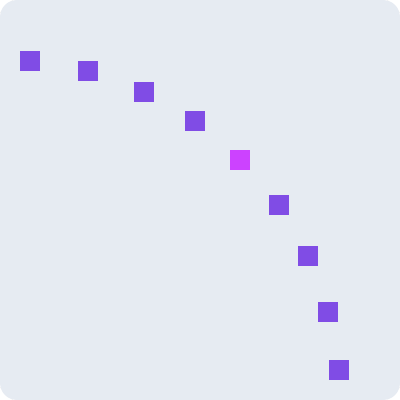
\includegraphics[width=11cm]{src/1.png}
\end{center}
\newpage
\Large{\textbf{Algoritmo de Rotación de una Linea}}\\[-0.4cm]
\begin{center}
\begin{mycodeboxl}
\begin{lstlisting}
from OpenGL.GL import *
from OpenGL.GLUT import *
from OpenGL.GLU import *
import numpy as np
import math

# Variables globales para los puntos
x1 = 350
y1 = 350
x2 = 50
y2 = 50
def punto():
    glColor3f(0.8, 0.26, 1.0)
    glLineWidth(3)
    glBegin(GL_LINES)
    glVertex2f(x1, y1)  # Coordenadas del punto inicial
    glVertex2f(x2, y2)  # Coordenadas del punto final
    glEnd()
def punto_rotacion(x1, y1,x2, y2, angulo):
    glColor3f(0.5, 0.3, 0.9)
    matriz_a = np.array([[math.cos(math.radians(angulo)), -math.sin(math.radians(angulo))],[math.sin(math.radians(angulo)), math.cos(math.radians(angulo))]])
    matriz_b = np.array([[x1], [y1]])
    matriz_c = np.array([[x2], [y2]])
    # Multiplicamos las matrices
    resultado1 = np.dot(matriz_a, matriz_b)
    resultado2 = np.dot(matriz_a, matriz_c)
    glBegin(GL_LINES)

    # Coordenadas del punto inicial rotado
    glVertex2f(resultado1[0], resultado1[1])  
    # Coordenadas del punto final rotado 
    glVertex2f(resultado2[0], resultado2[1])
    glEnd()
\end{lstlisting}
\end{mycodeboxl}
\end{center}
% -------------------------------------------------------------------

\begin{center}
\begin{mycodebox}
\begin{lstlisting}
def display():
    glClear(GL_COLOR_BUFFER_BIT)
    punto()
    punto_rotacion(x1, y1, x2, y2, -40)
    punto_rotacion(x1, y1, x2, y2, -30)
    punto_rotacion(x1, y1, x2, y2, -20)
    punto_rotacion(x1, y1, x2, y2, -10)
    punto_rotacion(x1, y1, x2, y2, 10)
    punto_rotacion(x1, y1, x2, y2, 20)
    punto_rotacion(x1, y1, x2, y2, 30)
    punto_rotacion(x1, y1, x2, y2, 40)
    glutSwapBuffers()

def main():
    # Declarar x y y como globales para poder modificarlas
    global x, y  
    glutInit(sys.argv)
    glutInitDisplayMode(GLUT_DOUBLE | GLUT_RGB)
    glutInitWindowSize(500, 400)
    glutInitWindowPosition(100, 100)
    glutCreateWindow("Dibujar Punto rotada")
    glClearColor(0.9, 0.92, 0.95, 1.0)
    gluOrtho2D(0.0, 499.0, 0.0, 499.0)
    glutDisplayFunc(display)
    glutMainLoop()

if __name__ == "__main__":
    main()
\end{lstlisting}
\end{mycodebox}
\end{center}
% -------------------------------------------------------------------
\newpage
Gráfico generado\\
\begin{center}

\includegraphics[width=16cm]{src/3.png}
\end{center}
\newpage


\Large{\textbf{Algoritmo de Rotación de la figura E}}\\
Se usará la matriz de coordenadas de la figura E presentada en el anterior informe
\begin{center}
\begin{mycodeboxl}
\begin{lstlisting}
from OpenGL.GL import *
from OpenGL.GLUT import *
from OpenGL.GLU import *
import numpy as np
import math

# Matriz de coordenadas del dibujo original
matriz_origen = [[200, 300, 300, 300, 300, 280, 200, 280],
[200, 290, 230, 290, 230, 180, 200, 180],
[200, 250, 260, 250, 260, 230, 200, 230],
[200, 200, 300, 200, 300, 180, 200, 180]]

def dibujar_E():
    glBegin(GL_QUADS)
    glColor3f(0.8, 0.26, 1.0)
    glVertex2f(matriz_origen[0][0],matriz_origen[0][1])
    glVertex2f(matriz_origen[0][2],matriz_origen[0][3])
    glVertex2f(matriz_origen[0][4],matriz_origen[0][5])
    glVertex2f(matriz_origen[0][6],matriz_origen[0][7])

    glVertex2f(matriz_origen[1][0],matriz_origen[1][1])
    glVertex2f(matriz_origen[1][2],matriz_origen[1][3])
    glVertex2f(matriz_origen[1][4],matriz_origen[1][5])
    glVertex2f(matriz_origen[1][6],matriz_origen[1][7])

\end{lstlisting}
\end{mycodeboxl}
\end{center}
% -------------------------------------------------------------------
\newpage

\begin{center}
\begin{mycodeboxl}
\begin{lstlisting}
    glVertex2f(matriz_origen[2][0],matriz_origen[2][1])
    glVertex2f(matriz_origen[2][2],matriz_origen[2][3])
    glVertex2f(matriz_origen[2][4],matriz_origen[2][5])
    glVertex2f(matriz_origen[2][6],matriz_origen[2][7])

    glVertex2f(matriz_origen[3][0],matriz_origen[3][1])
    glVertex2f(matriz_origen[3][2],matriz_origen[3][3])
    glVertex2f(matriz_origen[3][4],matriz_origen[3][5])
    glVertex2f(matriz_origen[3][6],matriz_origen[3][7])
    glEnd()

def punto_rotacion(angulo):
    glColor3f(0.5, 0.3, 0.9)
    # Matriz de rotación
    matriz_a = np.array([[math.cos(math.radians(angulo)), -math.sin(math.radians(angulo))], [math.sin(math.radians(angulo)), math.cos(math.radians(angulo))]])
    # Ubicando cada punto como matriz 
    matriz_b = np.array([[matriz_origen[0][0]], [matriz_origen[0][1]]])
    matriz_c = np.array([[matriz_origen[0][2]], [matriz_origen[0][3]]])
    matriz_d = np.array([[matriz_origen[0][4]], [matriz_origen[0][5]]])
    matriz_e = np.array([[matriz_origen[0][6]], [matriz_origen[0][7]]])
\end{lstlisting}
\end{mycodeboxl}
\end{center}
\newpage
% -------------------------------------------------------------------
\begin{center}
\begin{mycodeboxl}
\begin{lstlisting}
    matriz_f = np.array([[matriz_origen[1][0]],[matriz_origen[1][1]]])
    matriz_g = np.array([[matriz_origen[1][2]],[matriz_origen[1][3]]])
    matriz_h = np.array([[matriz_origen[1][4]],[matriz_origen[1][5]]])
    matriz_i = np.array([[matriz_origen[1][6]],[matriz_origen[1][7]]])

    matriz_j = np.array([[matriz_origen[2][0]],[matriz_origen[2][1]]])
    matriz_k = np.array([[matriz_origen[2][2]],[matriz_origen[2][3]]])
    matriz_l = np.array([[matriz_origen[2][4]],[matriz_origen[2][5]]])
    matriz_m = np.array([[matriz_origen[2][6]],[matriz_origen[2][7]]])

    matriz_n = np.array([[matriz_origen[3][0]],[matriz_origen[3][1]]])
    matriz_o = np.array([[matriz_origen[3][2]],[matriz_origen[3][3]]])
    matriz_p = np.array([[matriz_origen[3][4]],[matriz_origen[3][5]]])
    matriz_q = np.array([[matriz_origen[3][6]],[matriz_origen[3][7]]])

    # Multiplicando cada matriz punto con la matriz de rotación 
    resultado1 = np.dot(matriz_a, matriz_b)
    resultado2 = np.dot(matriz_a, matriz_c)
    resultado3 = np.dot(matriz_a, matriz_d)
    resultado4 = np.dot(matriz_a, matriz_e)

    resultado5 = np.dot(matriz_a, matriz_f)
    resultado6 = np.dot(matriz_a, matriz_g)
    resultado7 = np.dot(matriz_a, matriz_h)
    resultado8 = np.dot(matriz_a, matriz_i)
\end{lstlisting}
\end{mycodeboxl}
\end{center}
\newpage
\begin{center}
\begin{mycodeboxl}
\begin{lstlisting}
    resultado9 = np.dot(matriz_a, matriz_j)
    resultado10 = np.dot(matriz_a, matriz_k)
    resultado11 = np.dot(matriz_a, matriz_l)
    resultado12 = np.dot(matriz_a, matriz_m)

    resultado13 = np.dot(matriz_a, matriz_n)
    resultado14 = np.dot(matriz_a, matriz_o)
    resultado15 = np.dot(matriz_a, matriz_p)
    resultado16 = np.dot(matriz_a, matriz_q)

    # Dibujando la figura rotada
    glBegin(GL_QUADS)
    glVertex2f(resultado1[0], resultado1[1])  
    glVertex2f(resultado2[0], resultado2[1])  
    glVertex2f(resultado3[0], resultado3[1])  
    glVertex2f(resultado4[0], resultado4[1])  

    glVertex2f(resultado5[0], resultado5[1])  
    glVertex2f(resultado6[0], resultado6[1])  
    glVertex2f(resultado7[0], resultado7[1])  
    glVertex2f(resultado8[0], resultado8[1])  
    
    glVertex2f(resultado9[0], resultado9[1])  
    glVertex2f(resultado10[0], resultado10[1])
    glVertex2f(resultado11[0], resultado11[1])
    glVertex2f(resultado12[0], resultado12[1])

    glVertex2f(resultado13[0], resultado13[1])
    glVertex2f(resultado14[0], resultado14[1])
    glVertex2f(resultado15[0], resultado15[1])
    glVertex2f(resultado16[0], resultado16[1])

    glEnd()
\end{lstlisting}
\end{mycodeboxl}
\end{center}
\newpage
\begin{center}
\begin{mycodeboxl}
\begin{lstlisting}
def display():
    glClear(GL_COLOR_BUFFER_BIT)
    dibujar_E()
    punto_rotacion(-20)
    glutSwapBuffers()

def main():
    glutInit(sys.argv)
    glutInitDisplayMode(GLUT_DOUBLE | GLUT_RGB)
    glutInitWindowSize(500, 400)  # Tamaño de la ventana
    glutInitWindowPosition(100, 100)
    glutCreateWindow("Dibujar figura E rotada")
    glClearColor(0.9, 0.92, 0.95, 1.0)
    gluOrtho2D(0.0, 499.0, 0.0, 399.0)
    glutDisplayFunc(display)
    glutMainLoop()

if __name__ == "__main__":
    main()
\end{lstlisting}
\end{mycodeboxl}
\end{center}
Gráfico generado\\
\begin{center}

\includegraphics[width=13cm]{src/2.png}
\end{center}
\newpage

\end{document}
